\documentclass[dvipdfmx]{jsarticle}
\usepackage{ulem} %%下線、二重下線で使用
\usepackage{multirow} %%作表で使用する場合あり
\usepackage{graphicx} %%図版の貼り付けに使用
\usepackage{here} %%図版の貼り付けに使用
\usepackage{multicol} %%マルチカラムに使用
\usepackage{subcaption} %%2カラムの写真表示に使用
\usepackage{longtable}
\usepackage{booktabs}
\usepackage{tabularx}
\usepackage{url}
%%ソースリストの貼り付けに使用
\usepackage[utf8]{inputenc}
\usepackage[ipaex]{pxchfon}
\usepackage{amsmath} %%pmatrixに使用
\usepackage{svg}

\usepackage{listings}
% listings パッケージの設定
\lstset{
    language=Bash,
    basicstyle=\ttfamily\small,
    numbers=left,
    stepnumber=1,
    numbersep=5pt,
    showspaces=false,
    showstringspaces=false,
    showtabs=false,
    frame=single,
    tabsize=2,
    captionpos=b,
    breaklines=true,
    breakatwhitespace=false,
    columns=flexible,
    keepspaces=true,
    literate={"}{\texttt{"}}1
}

\begin{document}

\begin{titlepage}

\begin{flushright}
\begin{tabular}{|c|c|c|c|}
\hline
受付 & 月　日 & 評価 & \;\;\;\;\\
\hline
\end{tabular}
\end{flushright}


\begin{center}
    \vspace{100truept}

    \Huge 情報知能・工学実験　報告書

    \begin{tabular}{ |c|c| } 
    \hline
    実験題目 &  \\ 
    \hline
    \end{tabular}

    \vspace{30truept}

    {\normalsize
    \begin{tabular}{ |c|c| } 
    \hline
    実験実施日 &  令和 年 月 日 \\
    \hline
    第1回 &  令和 年 月 日 \\
    \hline
    第2回 &  令和 年 月 日 \\
    \hline
    第3回 &  令和 年 月 日 \\
    \hline
    第4回 &  令和 年 月 日 \\
    \hline
    第5回 &  令和 年 月 日 \\
    \hline
    第6回 &  令和 年 月 日 \\
    \hline
    \end{tabular}
    }

    \vspace{30truept}

    {\normalsize
    \begin{tabular}{ |c|c| } 
    \hline
    学籍番号 & 氏名 \\ 
    \hline
     &  \\ 
    \hline
    \end{tabular}
    }

    \vspace{30truept}

    {\normalsize
    \begin{tabular}{ |c|c| } 
    \hline
    概要 &  \\ 
    \hline
    \end{tabular}
    }
\end{center}

\end{titlepage}

\newpage

\section{目的}
近年のネットワーク技術の発展によりWebサービスが日常において不可欠な技術となっている。そのため、Webサービスの停止そのものが社会に与える影響が大きい。Webサービスの停止は外部からの攻撃によって起こされることがある。その種類は様々であるが、一つに「DoS攻撃」というものがある。DoS攻撃はセキュリティの脆弱なコンピュータに対して使用される。DoS攻撃をされたコンピュータはロードが急増し、サービスの提供が阻害されてしまうことが発生する。攻撃されたサービス事業者はこの攻撃によって得られる報酬が低減してしまう。よってWebサービスを運営するにあたってDoS攻撃の対策は必要不可欠である。

本実験において、ネットワークの基本構造について知り、DoS攻撃に対する対策法を身に着けることを目的とする。

\section{解説}
\subsection{DoS攻撃について}
DoS(Denial-of-Service)攻撃は特定のサーバやネットワークデバイスのwebサービスを停止させる攻撃手段の一つである。\\
DoS攻撃の一つにDDoS(distributed Denial-of-Service)攻撃がある。DDoS攻撃は、たくさんのコンピュータが同時に攻撃するプログラムを特定のサーバに対して実行する攻撃方法である。

Dos攻撃の方法には、サーバの脆弱性を悪用する攻撃とサーバに過負荷をかける攻撃の2つがある。サーバに脆弱性がある場合は、攻撃者に技術的なアドバンテージを利用されることによって攻撃を仕掛けられる。ただし、脆弱性を悪用する攻撃はソフトウェアのアップデートによって防ぐことができる。サーバに過負荷をかける攻撃は、意図的に通信手段をブロックすることやサーバが処理しきられないほどのロードをすることによってネットワークを混雑させることができる。そのため、ネットワークとサーバの間を無駄なパケットで埋め尽くすので、対策をサーバ内で施すことは難しいとされている。一方で、サーバ側ができる対策としてはファイヤーウォールを設定するという方法がある。

いかに様々なDos攻撃について記述する。

\subsubsection{UDP Flood}
通信プロトコルの一つであるUDPの特性を悪用する攻撃方法である。
長時間に大量のUDPパケットを送信することで攻撃を実行する。

\subsubsection{Ping Flood}
通信情報を取得するプロトコルICMPを悪用する攻撃方法である。
大量のICMPパケットを送り付けることによって攻撃する。

\subsubsection{SYN Flood}
TCP通信を確立するSYNを大量に送りつける攻撃方法である。
受信側の攻撃対象のサーバはSYNパケットを送り返した際にACKをタイムアウトまで待ち続けなければならないため、メモリを消費してしまうという攻撃方法である。

\subsubsection{Connection Flood}
コネクションが確立した状態を長時間つづけることでソケットを占有する攻撃方法である。

\subsubsection{HTTP GET Flood}
TCPコネクションが確立したのちにHTTP GETリクエストを大量に送信する攻撃方法である。シンプルな攻撃手段としてF5攻撃がある。F5はブラウザ上で押下することでwebページをリロードすることが可能であり、HTTP GETを短時間で大量に送ることが可能である。

\subsection{仮想マシンについて}
仮想マシンはコンピュータの操作をエミュレートするソフトウェアであり、この技術を使うことで一つの物理コンピュータで複数のOSを扱うことが可能となる。
例えば、Windows OS上でLinux OSの環境を構築することが可能なる。
webサービスはここ数年で大規模化され、それに伴いコストカットが重要となった。
そこで、コストの軽減のために一つのコンピュータで複数のOSを扱えるような仮想マシンの技術が開発された。

仮想マシンを動かすためのソフトウェアをVMM(Virtual Machine Monitor0)と呼ぶ。
VMMにはホスト型VMMとハイパーバイザ型VMMの2種類がある。
ホスト型VMMはホストOS上で実行され、ハイパーバイザ型VMMはインストールと実行が直接ハードウェア上で実行されるVMMである。
ここで、ハードウェアに直接ダウンロードされたOSをホストOSと呼ぶ。
ホスト型VMMはアプリケーションとして扱うことができるため、インストールや使い方が簡単である。一方、ハイパーバイザ型VMMはハードウェアとの間のレイヤーがホスト型よりも少ないため、実行時のオーバヘッドが少なくなる。一般的なVMMとして、VirtualBoxやVMwareはホスト型、KVM(Kernel-based Virtual Machine)はハイパーバイザ型である。本実験では、ハイパーバイザ型を使用する。

\section{実験環境}

本実験で使用したWebサーバのスペックを以下の表\ref{tab:WebServerSpec}に示す。\\
ここで、CPUのスペックの確認のコマンドは"lscpu"、メモリのスペックの確認のコマンドは"free -h"、ストレージのスペックの確認のコマンドは"lsblk"、ネットワークのスペックの確認のコマンドは"ip addr"、OSのスペックの確認のコマンドは"cat /etc/os-release"を使用した。

\begin{table}[H]
    \centering
    \caption{Webサーバのスペック}
    \label{tab:WebServerSpec}
    \begin{tabular}{|c|c|}
        \hline
        CPU & 1コア 3.4GHz \\
        \hline
        メモリ & 500MB \\
        \hline
        ストレージ & 7.6GB \\
        \hline
        IPアドレス & 192.168.1.197 \\
        \hline
        OS & Debian GNU/Linux 7 \\
        \hline
    \end{tabular}
\end{table}

本実験で使用した攻撃用サーバのスペックを以下の表\ref{tab:AttackerServerSpec}に示す。

\begin{table}[H]
    \centering
    \caption{攻撃用サーバのスペック}
    \label{tab:AttackerServerSpec}
    \begin{tabular}{|c|c|}
        \hline
        CPU & 1コア 3.4GHz \\
        \hline
        メモリ & 500MB \\
        \hline
        ストレージ & 8GB \\
        \hline
        IPアドレス & 192.168.2.198 \\
        \hline
        OS & Debian GNU/Linux 7 \\
        \hline
    \end{tabular}
\end{table}

また、攻撃用サーバにおいては、一つのサーバ内に複数のIPアドレスを生成するためセカンダリIPアドレスが、"192.198.197.1"から"192.198.197.150"まで生成されている。

実験に使用する攻撃ツールとして、"curl-loader"を使用する。
curl-loaderはC言語で書かれたWebアプリケーションに対する攻撃ツールの一つである。
一つのマシン上で複数のIPアドレスを使用して、リクエストの再生成を行うDDoS攻撃の一つである。

\section{実験課題}
\subsection{基礎実験} \label{sec:basicexperiment}
curl-loaderの実行時にパラメータを変更し、CPUの使用率、メモリの使用率、アクセスログ、などを調査する。
本実験では最初に環境を初期化するために、攻撃対象のwebサーバを再起動する。その際のコマンドを以下のソースリスト\ref{lst:restart}に示す。
\begin{center}
    ソースリスト\ref{lst:restart}：攻撃対象のwebサーバの再起動コマンド
\end{center}
\begin{lstlisting}[language=Bash, label={lst:restart}]
$ sudo /etc/init.d/apache2 restart
\end{lstlisting}

また、実験前にキャッシュをクリアするために、以下のソースリスト\ref{lst:clearcache}のコマンドを実行する。
\begin{center}
    ソースリスト\ref{lst:clearcache}：キャッシュクリアコマンド
\end{center}
\begin{lstlisting}[language=Bash, label={lst:clearcache}]
$ sudo sysctl -w vm.drop_caches=3
\end{lstlisting}

サーバの状態を観測するのにtopコマンドとapacheのアクセスログを使用する。
topコマンドは以下のソースリスト\ref{lst:top}のように引数を設定することができる。

\begin{center}
    ソースリスト\ref{lst:top}：topコマンドの引数設定
\end{center}
\begin{lstlisting}[language=Bash, label={lst:top}]
$ sudo top -b -d 1 -n 180 > top.log
\end{lstlisting}

このコマンドは、topコマンドをバッチモードで実行し、1秒ごとに180回の更新を行い、その結果をtop.logに出力するものである。
こうすることで、サーバの状態を1秒おきに観測することができる。

topコマンドからCPUの使用室のみを抽出しファイルに書き出すコマンドを以下のソースリスト\ref{lst:extractcpu}に示す。
\begin{center}
    ソースリスト\ref{lst:extractcpu}：CPU使用率の抽出コマンド
\end{center}
\begin{lstlisting}[language=Bash, label={lst:extractcpu}]
$ grep "%Cpu" top.log | awk '{print $2}' > cpu.log
\end{lstlisting}

topコマンドからメモリの使用率のみを抽出しファイルに書き出すコマンドを以下のソースリスト\ref{lst:extractmem}に示す。
\begin{center}
    ソースリスト\ref{lst:extractmem}：メモリ使用率の抽出コマンド
\end{center}
\begin{lstlisting}[language=Bash, label={lst:extractmem}]
$ grep "Mem" top.log | awk '{print $5/$3}' > mem.log
\end{lstlisting}

access.logから1秒ごとのアクセス数を抽出してファイルに書き出すコマンドを以下のソースリスト\ref{lst:extractaccess}に示す。
\begin{center}
    ソースリスト\ref{lst:extractaccess}：アクセス数の抽出コマンド
\end{center}
\begin{lstlisting}[language=Bash, label={lst:extractaccess}]
$ grep "192.168.197." access.log | awk '{print $4}' | sort | uniq -c > freq.log
\end{lstlisting}

本実験では、curl-loaderの設定ファイルであるsample.cnfの"TIMER\_AFTER\_URL\_SLEEP"の値を200, 400, 800に変更してその結果を比較する。
この時、"TIMER\_AFTER\_URL\_SLEEP"はリクエストの完了後に次のリクエストをするまでcurl-loaderが待機する時間をミリセカンド単位で表すパラメータである。

curl-loaderの実行コマンドは以下のようになる。
\begin{lstlisting}[language=Bash]
$ sudo curl-loader -f sample.cnf
\end{lstlisting}

curl-loaderはroot権限を持ったうえで実行しなければならない。
ただし、\&によってコマンドをつなぐことは後続のコマンドもroot権限で実行されてしまうため、注意が必要である。

\subsection{攻撃者判定実験}

攻撃者を検知してフィルタリングするシェルスクリプトをwebサーバ上で作成する。
加えて、\ref{sec:basicexperiment}で行った実験をもう一度行い、フィルタリング設定時のふるまいを調査する。
その際に以下の箇条書きの点を満たすように調査する。
\begin{itemize}
    \item TIMER\_AFTER\_URL\_SLEEPの値を100, 200, 400に変更した際のCPU使用率、メモリ使用率、アクセスログを測定する。
    \item フィルタリングをかけた時と書けない時の値を測定する。
    \item iptableのDROPに基づいてフィルタリングを行う。
    \item フィルタリングする攻撃者の基準として、毎秒三回以上アクセスしているIPアドレスに絞るようにする。
    \item 攻撃者の見地は"/var/log/apache2/p3/access.log"のアクセスログをもとに判断する。
\end{itemize}

また、Webサーバのホームディレクトリ上に"attecker\_search"というディレクトリを作成し、攻撃者の判定に使用したフィルを保存する。

\section{実験結果}
\subsection{基礎実験}
最初に、apacheを再起動した際のコマンドの実行結果とキャッシュをクリアした際のコマンドの実行結果を以下のソースリスト\ref{lst:initresult}に示す。
\begin{center}
    ソースリスト\ref{lst:initresult}：攻撃対象のwebサーバの初期化コマンドの実行結果
\end{center}
\begin{lstlisting}[language=Bash, label={lst:initresult}]
$ sudo /etc/init.d/apache2 restart
[ ok ] Restarting apache2: apache2 ... waiting .
$ sudo sysctl -w vm.drop_caches=3
vm.drop_caches = 3
\end{lstlisting}

以下の図\ref{fig:cpu_exp1}にTIMER\_AFTER\_URL\_SLEEPの値を200, 400, 800に変更した際のCPU使用率のグラフを示す。
\begin{figure}[H]
    \centering
    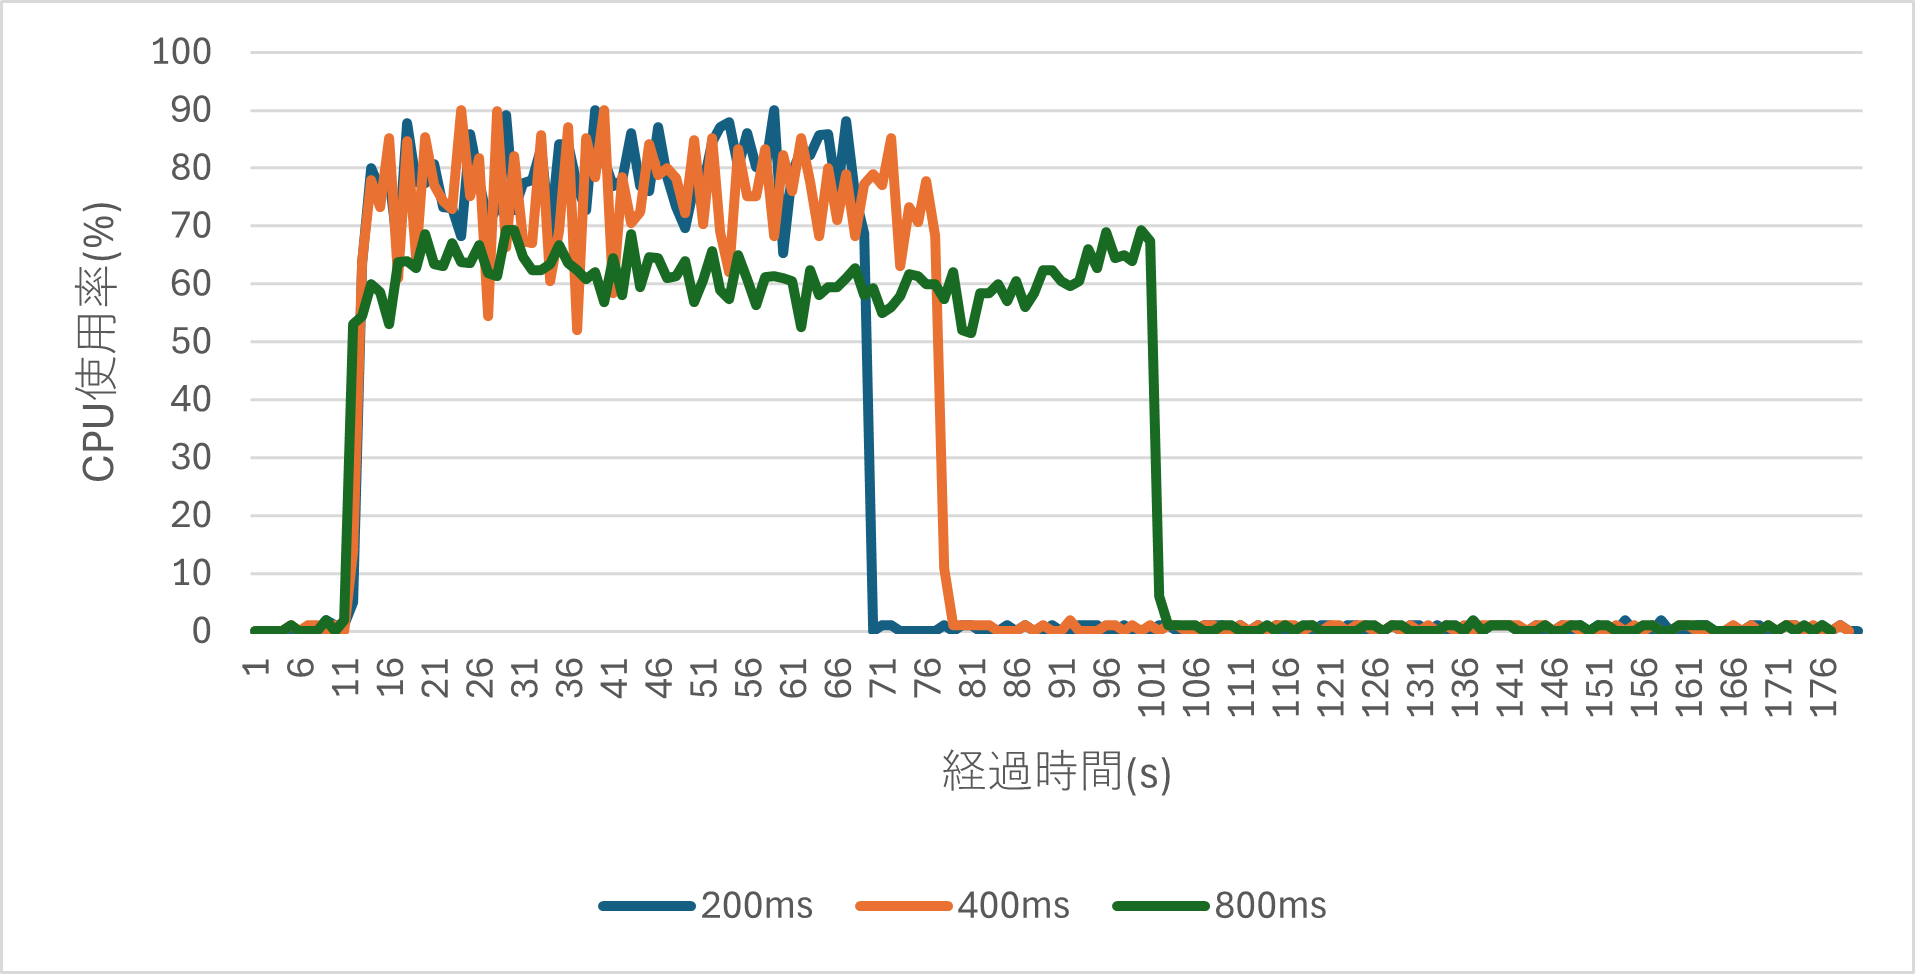
\includegraphics[width=0.8\textwidth]{images/exp1/cpu2.png}
    \caption{基礎実験のCPU使用率のグラフ}
    \label{fig:cpu_exp1}
\end{figure}

以下の図\ref{fig:mem_exp1}にTIMER\_AFTER\_URL\_SLEEPの値を200, 400, 800に変更した際のメモリ使用率のグラフを示す。
\begin{figure}[H]
    \centering
    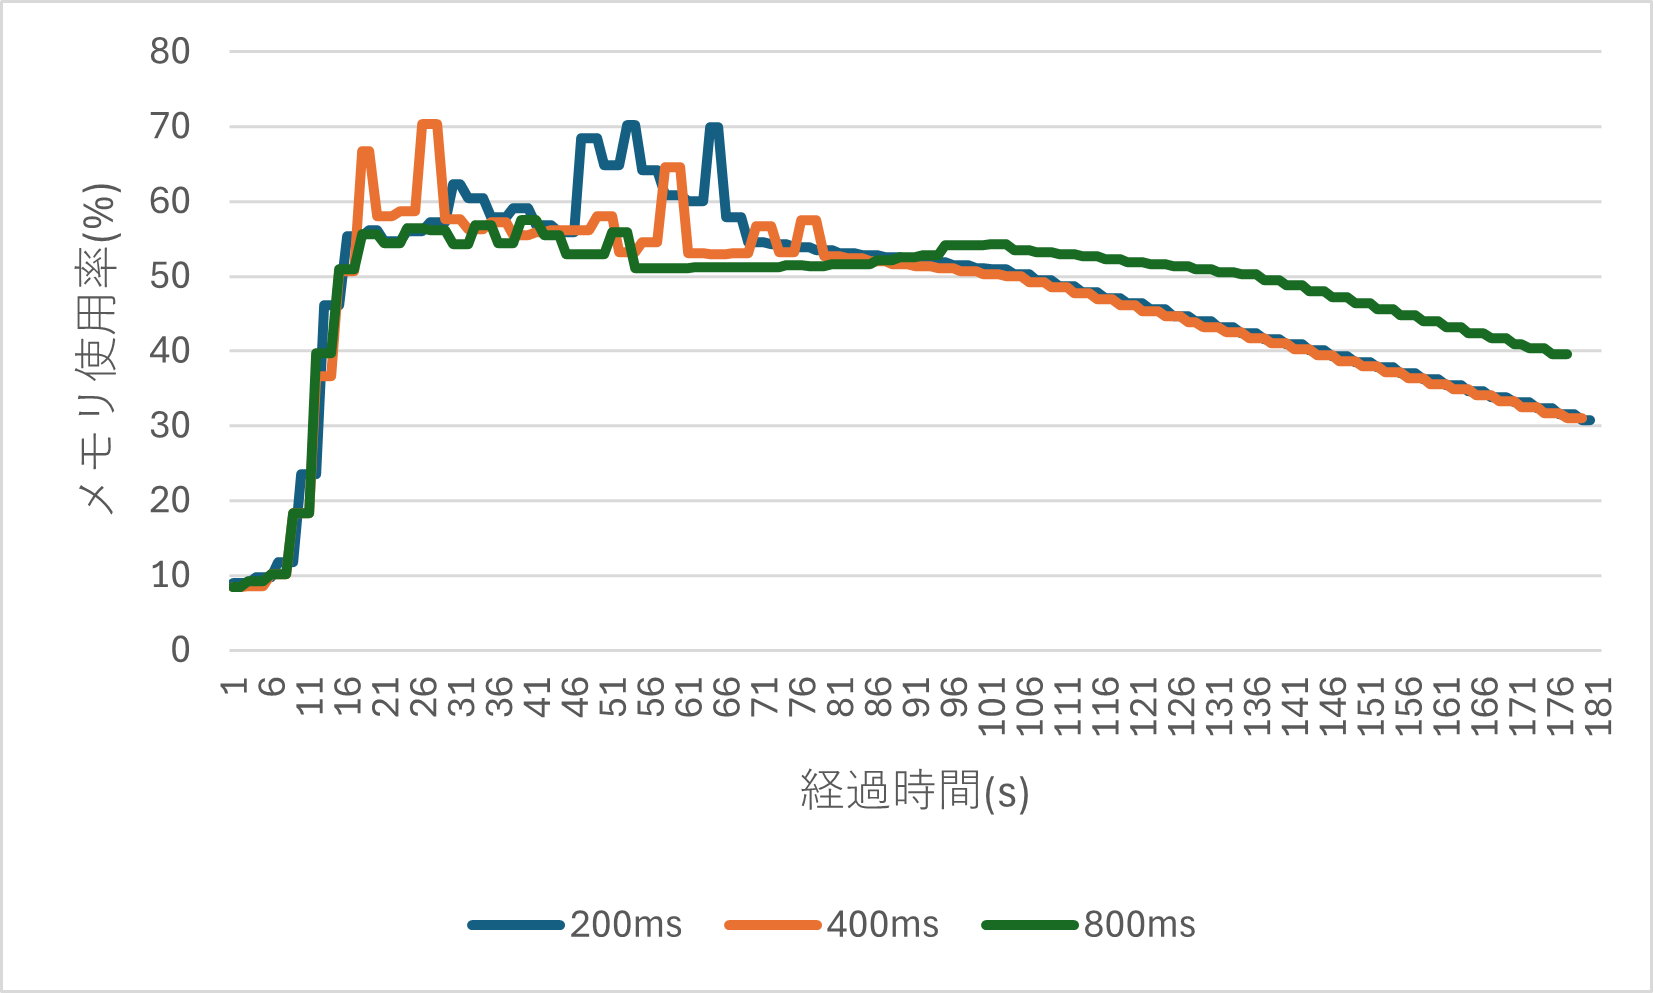
\includegraphics[width=0.8\textwidth]{images/exp1/mem2.png}
    \caption{基礎実験のメモリ使用率のグラフ}
    \label{fig:mem_exp1}
\end{figure}

以下の図\ref{fig:access_exp1}にTIMER\_AFTER\_URL\_SLEEPの値を200, 400, 800に変更した際のアクセス数のグラフを示す。
\begin{figure}[H]
    \centering
    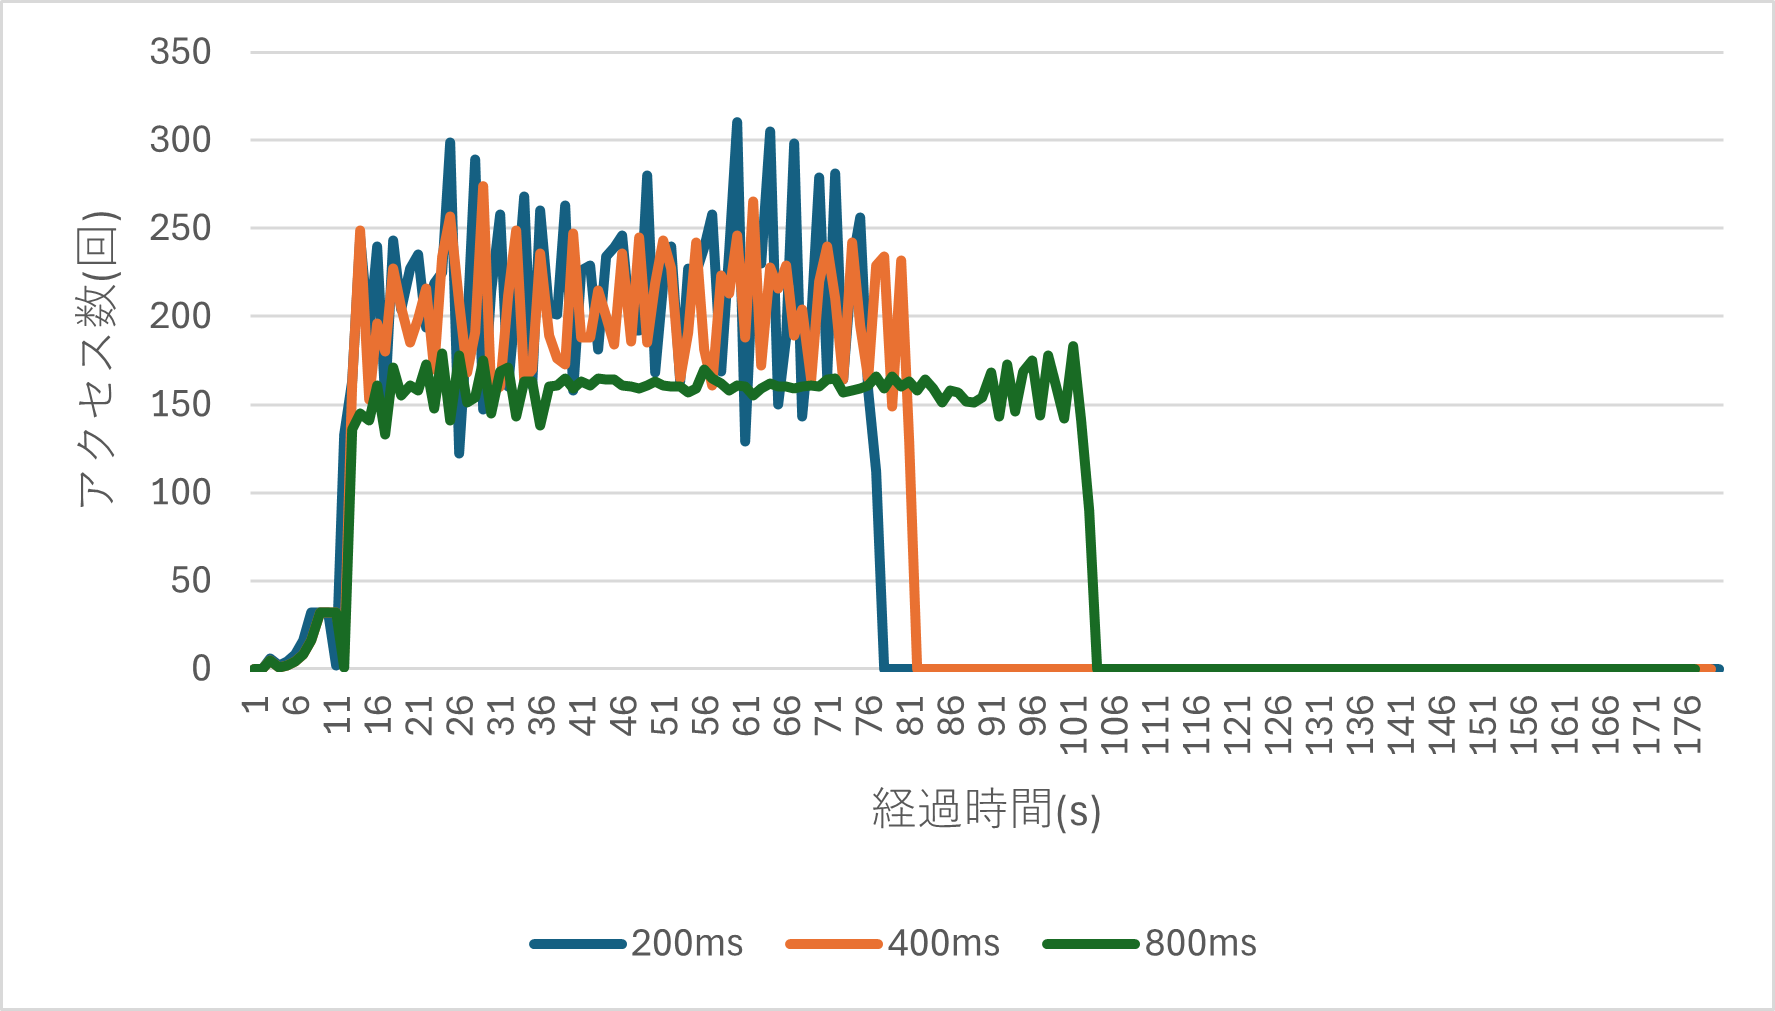
\includegraphics[width=0.8\textwidth]{images/exp1/freq2.png}
    \caption{基礎実験のアクセス数のグラフ}
    \label{fig:access_exp1}
\end{figure}

図\ref{fig:cpu_exp1}において、グラフのうち変化率が最大になった後はCPU使用率が50\%を超える時間が続き、変化率が最小になった後はCPU使用率が5\%を下回る時間が続いていることがわかる。よって、攻撃によってCPUに負荷がかかっているのは、CPU使用率が50\%を超える時間帯であると考えられる。\\
また、CPU使用率が50\%を超える時間帯において、TIMER\_AFTER\_URL\_SLEEPの値が200と400の時のCPU使用率は、800の時よりも高い時間が長いことがわかる。また、TIMER\_AFTER\_URL\_SLEEPの値が大きいほどCPUの使用率が50\%を超える時間が長くなっていることがわかる。よって、TIMER\_AFTER\_URL\_SLEEPの値が小さいほどCPU使用率への影響が大きく、値が大きいほど攻撃の影響が長く続くことがわかる。\\

図\ref{fig:mem_exp1}において、グラフのうち変化率が大きくなったのちにメモリ使用率が0.5を超える時間が続き、CPU使用率が5\%を下回っている時間において変化率が徐々に小さくなっていることがわかる。攻撃の受け始めの変化率がCPU使用率よりもなだらか上昇している。また、CPU使用率は攻撃が終わると1秒間で50\%以上の値から5\%以下の値に減少するのに対して、メモリ使用率は、20秒以上経過したのちにで10\%減少するので、CPU使用率よりもなだらかに減少していることがわかる。よって、攻撃によってメモリに負荷がかかっているのは、メモリ使用率が0.5を超える時間帯であると考えられる。\\

図\ref{fig:freq_exp1}において、グラフのうち変化率が最大になった後はアクセス数が100回を超える時間が続き、変化率が最小になった後はアクセス数が5回を下回る時間が続いていることがわかる。よって、攻撃によってアクセス数に影響がかかっているのは、アクセス数が100回を超える時間帯であると考えられる。\\
また、アクセス数が100回を超える時間帯において、TIMER\_AFTER\_URL\_SLEEPの値が200と400の時のアクセス数は、800の時よりも高い時間が長いことがわかる。また、TIMER\_AFTER\_URL\_SLEEPの値が大きいほどアクセス数が50\%を超える時間が長くなっていることがわかる。よって、TIMER\_AFTER\_URL\_SLEEPの値が小さいほどアクセス数への影響が大きく、値が大きいほど攻撃の影響が長く続くことがわかる。\\

図\ref{fig:cpu_exp1}、図\ref{fig:freq_exp1}より、CPU使用率とアクセス数の増加率が最大のタイミングと最小のタイミングが同じであることがわかる。よって、攻撃によってアクセス数が増えること自体がCPU使用率の増加に影響していると考えられる。対して、メモリ使用率は増加率の増え方がなめらかであり、増加はCPUの使用率が50\%以上になった時間よりも先に始まっていることから、攻撃によってアクセス数が増えたタイミングでapacheが複数のタスクの処理をするためにメモリをたくさん確保し、その後CPUがそのタスクを処理しているため、CPUの使用率がメモリの使用率の増加よりも遅れていると考えられる。





\subsection{攻撃者判定実験}

\section{調査課題}


\pagebreak
\begin{thebibliography}{9}
\end{thebibliography}

\end{document}
